% Template for PLoS
% Version 1.0 January 2009
%
% To compile to pdf, run:
% latex plos.template
% bibtex plos.template
% latex plos.template
% latex plos.template
% dvipdf plos.template

\documentclass[10pt]{article}

% amsmath package, useful for mathematical formulas
\usepackage{amsmath}
% amssymb package, useful for mathematical symbols
\usepackage{amssymb}

% graphicx package, useful for including eps and pdf graphics
% include graphics with the command \includegraphics
\usepackage{graphicx}

% cite package, to clean up citations in the main text. Do not remove.
\usepackage{cite}

\usepackage{color} 

% Use doublespacing - comment out for single spacing
%\usepackage{setspace} 
%\doublespacing

%FZ: Enable the comment command
\usepackage{verbatim}
% Text layout
\topmargin 0.0cm
\oddsidemargin 0.5cm
\evensidemargin 0.5cm
\textwidth 16cm 
\textheight 21cm

% Bold the 'Figure #' in the caption and separate it with a period
% Captions will be left justified
\usepackage[labelfont=bf,labelsep=period,justification=raggedright]{caption}

% Use the PLoS provided bibtex style
\bibliographystyle{plos2009}

% Remove brackets from numbering in List of References
\makeatletter
\renewcommand{\@biblabel}[1]{\quad#1.}
\makeatother


% Leave date blank
\date{}

\pagestyle{myheadings}
%% ** EDIT HERE **


%% ** EDIT HERE **
%% PLEASE INCLUDE ALL MACROS BELOW
\long\def\authornote#1{%
        \leavevmode\unskip\raisebox{-3.5pt}{\rlap{$\scriptstyle\diamond$}}%
        \marginpar{\raggedright\hbadness=10000
        \def\baselinestretch{0.8}\tiny
        \it #1\par}}
\newcommand{\bastian}[1]{\authornote{BG: #1}}
\newcommand{\fabian}[1]{\authornote{FZ: #1}}
\newcommand{\philipp}[1]{\authornote{PB: #1}}
%% END MACROS SECTION
\begin{document}

% Title must be 150 characters or less
\begin{flushleft}
{\Large
\textbf{openSNP - Crowdsourcing Genome-Wide Association Studies}
}
% Alternative titles: 
% openSNP - a new, open data-source for personalised medicine
% What kind of person would share genotyping-data? Presenting a survey and an open data-source for personalised medicine
% 
% Insert Author names, affiliations and corresponding author email.
\\
Bastian Greshake$^{1,\ast}$, 
Philipp Bayer$^{2}$, 
Fabian Zimmer$^{3}$,
Julia Reda$^{4}$
\\
\bf{1} Goethe University, Frankfurt am Main, Germany
\\
\bf{2} University of Queensland, Brisbane, Australia
\\
\bf{3} Westf\"alische Wilhelms Universit\"at, M\"unster, Germany
\\
\bf{4} Johannes-Gutenberg University, Mainz, Germany
\\
$\ast$ E-mail: info@opensnp.org
\end{flushleft}

% Please keep the abstract between 250 and 300 words
\section*{Abstract}
Genome-wide association studies are used to correlate phenotypic traits with genetic variants like Single Nucleotide Polymorphisms (SNPs). Genome-wide association studies compare the genetic variation between two groups to find correlations between membership in a group and the genetic variation. To find significant correlations it is necessary to have a large enough sample size. The advent of Direct-To-Consumer genetic testing offers the analysis of SNPs for an individual at low cost without the need to consult a physician or geneticist. Over 100,000 people have already been genotyped through Direct-To-Consumer genetic testing. This data could be a valuable source for association studies. However, this data is not public for various reasons and thus cannot be used by other scientists. It seems reasonable to create a central open data-repository for such data, but it was previously unknown if and how people would submit their data to such a repository. Here we present a survey which evaluates whether people are willing to publicly share their genetic information. In the light of those results we also present the web-platform openSNP, an open database which allows participants of Direct-To-Consumer genetic testing to publish their genetic data along with phenotypic information into the public domain. Through this "crowdsourced" effort of collecting genetic and phenotypic information we create a valuable resource which can be used in a wide array of studies, included Genome-wide association studies. OpenSNP is hosted at www.opensnp.org, and the code is released under MIT-license at github.com/gedankenstuecke/snpr.


% Please keep the Author Summary between 150 and 200 words
% Use first person. PLoS ONE authors please skip this step.
% Author Summary not valid for PLoS ONE submissions.   
\section*{Author Summary}
Missing for now.

\section*{Introduction}

The availability of new DNA sequencing techniques has shifted the focus of biological data acquisition towards new biomedical applications.
Many diseases – for example Alzheimers, Parkinsons or different types of cancers – are at least partially heritable so the genome 
of patients can be used for diagnostic purposes. Using the genetic information of patients is made possible through the sharp decrease in costs for analysing genetic information. 

%Kicked out the following due to Corpas' argument
%The comparison of DNA sequences from individuals in a population can reveal variable sites, which are of major interest in investigating diseases. 
%A variation of only one nucleotide length at a given site is called a single Nucleotide Polymorphisms (SNP). 
%The different nucleotides at this site are defined as an allele.
%For diploid organisms, as us humans, the genotype at a given site consists of two alleles, which are independently inherited from each parent.
%Different methods have been developed to read SNPs in an individual, a
%process called genotyping. A widespread used method for genotyping individuals is the use of microarrays.
%In comparison to whole genome sequencing only sites which are known to be variable are analysed, making microarrays cheaper and faster \cite{Brown1999}. 


If the genotypes for more than one individual are known, the analysis of
allele frequencies can be used to associate SNPs with diseases and other inheritable traits. Genome-Wide Assocation Studies
(GWAS) make use of statistics to compare the alleles of patients to the alleles of healthy controls. This
enables GWAS to find alleles which are significantly overrepresented in patients and associate them with a disease.
This method does not allow inference of causal differences but merely identifies correlations. 
The first GWAS was published in 2005 and compared age-related macular degeneration in contrast 
to a healthy control group \cite{Klein2005}. Since the beginning, the number of participants in 
such studies has been rising. To date, over 1200 GWAS have been performed \cite{Johnson2009} and over 
5000 SNPs have been linked to different diseases and traits \cite{Hindorff2009}. 
%(http://www.genome.gov/page.cfm?pageid=26525384&clearquery=1#result_table)  

GWAS are not limited to the scientific community. Since 2006, companies like 23andMe, deCODEme or FamilyTreeDNA have been offering Direct-To-Consumer (DTC) genetic testing. 
These companies use DNA microarrays to screen for around 0.5 to 1 million SNPs spread over the human genome. In return, customers 
receive an analysis of the results, as well as a file that includes the customer's raw individual genotypes. In 2011, 23andMe 
alone had over 100,000 customers \cite{23andMe2011}
- the company realizes the potential to perform GWAS with this amount of data by using surveys to ask their customers about 
traits and diseases. With the consent of the customer the data is used for association studies. 23andMe has published several 
articles in which known findings are replicated together with new associations disorders like Parkinson's Disease \cite{Eriksson2010, Do2011}. 
So far, over 30,000 23andme-customers have participated in 23andme's association studies, which proves that this data-source has a lot of potential for other researchers.

The generation of biomedical data by private companies raises concerns about privacy \cite{23andMe2012}, 
liability and consent \cite{Caulfield2011}. 
Nevertheless, in some instances individual customers are willingly sharing their data. Most do so by uploading their data to
their personal website or to open software repositories like \textit{GitHub}. 
This data is scattered and unorganized, making it hard to use. While projects like SNPedia try to keep track of all 
the publicly available genotyping files \cite{Cariaso2011}, they usually do not provide the information necessary to perform GWAS, as the phenotypic information is 
often not attached to the genetic information. Projects that attach the phenotype to the genetic information, 
like the \textit{Personal Genome Project}, still do not allow for an easy re-use of the data, as they lack an advanced programming interface (API) 
or other methods by which researchers could download the data. Additionally, not every customer of DTC genetic testing can participate in the \textit{Personal Genome Project}.  

Here, we present the results of a survey designed to evaluate the support in the personal genetics community for a crowdsourced online platform. 
We also present openSNP, an online platform which enables DTC customers to share genotypic and phenoytypic information, as well as receive additional information on their genotypes. 
The genotypes are made available to researchers via the open Creative-Commons-Zero licence.

% Results and Discussion can be combined.
\section*{Results}

\subsection*{Survey on Sharing Genetic Information}
In total 229 people, 180 with a self-reported chromosomal sex of XY and 56 with a self-reported chromosomal sex of XX participated in our survey on sharing genetic information with the public. 
The mean age of the participants is 33 (SD = 11,29). 81.7 \% reported their ethnicity as caucasian. 39.7 \% of the participants are already 
customers of at least one DTC genetic testing company and further 30.1 \% of them plan on becoming one in the future. 29.7 \% do not plan on 
becoming a DTC customer. There is no significant difference in the usage of DTC companies between chromosomal sexes (Cramer's V = 0.077). 

67.7 \% of all participants would share their data with their DTC-company without any constraints, 25.8 \% would do so given the company 
didn't share the data with third parties. 6.6 \% of the participants would not share their data. Participants self-identified as XX-chromosomal are slightly more likely to answer that DTC companies are allowed to use their results (Cramer's V = 0.221). Those who are customers of a DTC company or are planning on becoming one in 
the future are more likely to share their results, compared to those who do not plan on getting themselves genotyped (Somers-d = 0.331). 

There are substantial differences in terms of motivation, tested by Tukey's HSD test, between those people who have already been genotyped 
and those who are not planning on getting genotyped. The first group is likely to agree more strongly, on a five-point scale, with the following 
motivations for sharing genotypic information: because they want to help scientists (mean difference = 0.465, SE = 0.128), 
because they think of personal benefits (mean difference = 0.448, SE = 0.183) and because they are curious (mean difference = 1.159, SE = 0.193). 

On the other hand, those people who are not planning on getting genotyped are more likely to agree with the following motivations 
for not sharing their data: because they fear discrimination (mean difference = 1.060, SE = 0.195), because they feel 
it is a breach of their privacy (mean difference = 0.821, SE = 0.225), because they fear negative consequences for their 
family members (mean difference = 0.733, SE = 0.21) or because they fear personalized advertising (mean difference = 0.848, SE = 0.208).

Similarly, those people who would share data with their DTC provider under any circumstances are likely to agree more strongly with 
the following motivations for sharing than those who would not share their data with their DTC company: because they want to help 
scientists (mean difference = 1.57, SE = 0.199), because they think of personal benefits (mean difference = 0.951, SE = 0.308), 
and because they are curious (mean difference = 1.99, SE = 0.321). In the case of curiosity as a motive, there is also a substantial difference between those who would share their data with their DTC company under the condition that it did not share the information and those who would not (mean difference = 1.116 SE = 0.344) as well as those who would share under any circumstances (mean difference = -0.874 SE = 0.182).

Those participants who are not willing to share data with their DTC company are likely to agree more strongly with the following motivations 
for not sharing their data when compared to those who would share their data with their DTC company under any circumstances: because they 
fear discrimination (mean difference = 1.52, SE = 0.322), because they feel it is a breach of their privacy (mean difference = 1.871, SE = 0.324), 
because they fear consequences for their family members (mean difference = 1.146, SE = 0.32) and because they fear personalized advertising (mean difference =  1.112, SE = 0.357). In the cases of fear of discrimination and fear of a breach of privacy, substantial differences between all three categories exist. Those who would share their data with their DTC company as long as it did not share the information agree less strongly than those who would not share the data with both fear of discrimination as a motive for not sharing (mean difference = -0.615, SE = 0.345) as well as fear of a breach of privacy (mean difference = -0.668, SE = 0.346). Those who would share their data under any circumstances are even less likely to agree with these motives than those who would share only if their DTC company did not share the information (fear of discrimination: mean value = -0.906, SE = 0.182; breach of privacy: mean difference = -1.203, SE = 0.183).

\subsection*{openSNP}

The openSNP project (http://opensnp.org) is an open, crowdsourced online platform for both DTC customers and researchers interested in performing GWAS. 
DTC customers are encouraged to share their genotyping results and connect them with phenotypes to enable access for researchers.
Users can create a personal profile, discuss SNPs and phenotypes on the 
platform using a simple commenting system, or send each other private messages. 


\subsubsection*{Sharing genotypic information}
Currently users can upload their genotypings from the companies 23andme, deCODEme and FamilyTreeDNA via a webinterface to the openSNP 
project. There is experimental support for openSNP-exomes. The uploaded data is published under the Creative Commons Zero-license, 
which - in accordance with the Panton Principles (doi:10.1371/journal.pbio.1001195) - 
allows a complete reuse of the data without any constraints.
Between the start of openSNP on 09/27/2011 and 12/18/2012, 214 people have signed 
up with openSNP, and 79 genotyping files were made available. The openSNP 
database lists 69,486,471 SNPs of which 1,938,603 are unique SNPs.
Figure \ref{Figure1_label} depicts the increase of users and genotyping files over time.


\subsubsection*{Crowdsourcing phenotypes}
Users are able to create new phenotypes that are not yet 
listed by openSNP. 
The specification of these phenotypes is open and not limited 
to pre-defined categories. To reduce the amount of manual data curation, openSNP tries to harmonize 
the expression and spelling of the same phenotype or variation. We implemented an 
autocompletion-feature, which helps users to reuse already entered phenotypes.
Users are encouraged to list as many phenotypes as possible through a simple 
achievement system, rewarding users that upload their data and enter phenotypic 
information with small badges that are shown on their profile pages.

In the same timeframe as above, all users combined have 
entered a total of 675 variations on 47 different phenotypes with those variations being 
the different values on a given trait or phenotype. See figure \ref{Figure1_label} for the increase of phenotypic information over time.

The mean number of users that have entered their variations for a single phenotype 
is 14.36 (SD 12.65), the median is 10. The distribution of how many users have 
entered their data per phenotype can be seen in figure \ref{Figure2_label}. The phenotype provided 
by the most users is the eye color, which has been entered by 54 users. There are 
two phenotypes which have so far only been provided by a single user: 
the SAT Writing score and triglyceride-levels.


\subsubsection*{Connection to external services}
In order to provide users with relevant information on their respective genotypes, openSNP scans databases of the scientific literature for specific SNPs. 
A total number of 15,229 documents relevant to the SNP-IDs listed in openSNP could be found in the databases of Mendeley, the Public Library of Science and SNPedia. 
Of the primary literature, 25 \% are released in open access journals and can be accessed free of charge (Figure \ref{Figure3_label}). For usability reasons, 
SNPs are ranked by the amount of information gathered by the external services. The external services themselves are ranked by how easily non-scientists can understand information 
from these sources. The SNPedia entries are given the highest impact, as those are already manually curated and summarized in plain English, followed by open access publications out of 
the Public Library of Science. Lowest values are given to the Mendeley results, as those are not necessarily freely available to every user. 
An entry on SNPedia is valued 2.5 times as high as a PLoS publication and 5 times as high as a Mendeley entry.  

\subsubsection*{Data access}
OpenSNP offers extensive access to the data uploaded by users. Anyone can download single genotyping files for specific users, get archives of multiple genotyping files 
grouped by phenotypic variation, or access a single download that includes all genotyping files and all phenotypes in a comma-separated table. The genetic data is also 
accessible through the Distributed Annotation System \cite{Dowell2001,Jenkinson2008}, which offers all data for specific chromosomes and specific positions on single chromosomes. 
The data is additionally available over a JSON-API, which allows users to directly access data in the JSON-format.

\section*{Discussion}

\subsection*{Survey issues}
As the survey was taken online by voluntary participants and was mainly spread in the personal genetics community, 
the results do not reflect the general population, but over-represent those people most likely to be interested in
a project such as openSNP: customers of DTC genetic testing companies and people with a high interest in biology. 

\subsection*{Privacy, health implications and ethical considerations}

%The advent of DTC genetic testing has led to new ethical and social issues. 
Much of the critique on DTC genetic testing focusses on the practice 
of delivering medical information without consulting a physician or genetic counsellor to help patients/customers make sense of the information 
and to put the new knowledge to good use \cite{Hauskeller2011,Hogarth2008,Wasson2009}.  

As we have found in the survey on sharing such results, many DTC customers are willing to share their results with the public to help scientific progress, without forgetting about the privacy implications that come with openly sharing genetic information. There is a variety of ethical and privacy implications when it comes to DTC genetic testing\cite{Caulfield2011,Joh2011}. 

Our survey has shown that people are concerned about their privacy and fear that stakeholders like employers, insurance companies, governments 
or advertisers might misuse the information. Policy makers start to react to those changes by introducing laws like the 
\textit{Genetic Information Non-Discrimination Act} in the United States or the \emph{Gendiagnostikgesetz} in Germany to minimize the impact of
widely available genetic information. DTC genetic testing companies themselves also try to educate their customers about the risks of releasing genetic data.  

OpenSNP openly addresses the problem of privacy implications that come with releasing genetic data twice, once during registration for openSNP and once during 
the upload of the DTC genetic testing results. Users have to confirm that they have read and understood the disclaimer about possible side-effects 
of publishing their data. To further improve this process we are working on implementing an informed consent-processes 
similar to \textit{Consent for Research} (http://www.weconsent.us).

\subsection*{GWAS and open data}
Although prices of exome or even full genome sequencing are dropping rapidly, GWAS are still considerably cheaper. However, GWAS can only detect correlations of SNPs with those traits and do not allow 
inference on the cause for any correlation. Furthermore, for a statistically sound analysis GWAS need a large enough sample size. Nevertheless, GWAS are still frequently used and new associations are found \cite{10.1371.journal.pone.0031470,10.1371.journal.pone.0030309,10.1371.journal.pone.0029848}. 

One way of bringing down costs for GWAS even further is to make use of already available genotyping results and datasets. 
Data produced by DTC genetic testing companies is a promising source for such data, as such companies already have high 
numbers of customers which are willing to pay for the genotyping by themselves.

By crowdsourcing the acquisition of genetic and phenotypic data, openSNP faces the same problems as any other 
open platform on the Internet, namely the need to trust users regarding the data they upload and enter on openSNP. 
Additionally, the quality of the data varies, especially in terms of accuracy on the phenotypic variation, 
with users entering data in different measurement systems. Another problem with user-entered data is the frequent switching between categorical and continuous phenotypes - for example, some users entered the specific value of their height, while other users entered their height according to a category like "150cm to 160cm". 

While we try to suggest similar entries to the users, 
there are some cases where users will not follow those suggestions, so duplicates or similar phenotypes or variations in traits may arise. There are two possible solutions to this problem: The first one would be to only allow a trusted subset of users to enter new phenotypes. The other one 
would be to make users enter all possible variations of a phenotype while creating a new phenotype, so that later users cannot add 
variations that have not been available from the start. 

In both cases it makes it harder 
for users to enter their data which raises the bar for participation.
We decided to keep data entry as easy as possible, at the cost of forcing users who want to perform GWAS with the data to perform more quality control.

Another risk regarding data quality that should be kept in mind is a possible bias in data availability on openSNP: only a subset of people buy DTC genetic testing, from which an even smaller subset is willing to publish the results, which can potentially lead to skewed GWAS-results.

With openSNP, we have built a platform that can be used by customers of DTC genetic testing to easily share their genetic and phenotypic 
data with a wide audience, as well as by scientists and interested citizens who are looking for datasets to freely use in their studies.
Customers of DTC genetic testing also benefit from an easy access to primary literature on SNPs and genetic variations they carry. 
While there is not enough data uploaded to perform a statistically sound GWAS yet, this will be possible in the future, as user numbers continue to rise.

 
% You may title this section "Methods" or "Models". 
% "Models" is not a valid title for PLoS ONE authors. However, PLoS ONE
% authors may use "Analysis" 
\section*{Materials and Methods}
\subsection*{Survey on Sharing Genetic Information}
The survey was performed using Google Docs and was distributed to possible participants through the 23andMe community, the DIYBiology mailing list, 
blogs which focus on genetics and DTC genetic testing and social media like Twitter, Google Plus and Facebook.  

The survey included demographics such as age, chromosomal sex and ethnicity of the participants. Furthermore, it included questions on their 
(planned) customer-ship of a DTC company. If the participants already were customers, they were also asked if they were already sharing their genetic and phenotypic data. 
All participants were asked if they would share their genetical or phenotypic information with their DTC company, possible answers were "Yes", "Yes, 
but only if they did not share my medical information with anybody else" and No".

The survey also asked some scaled questions which measured how strongly participants agreed/disagreed with different reasons for sharing or not sharing their 
information. The scale went from 1 = strongly disagree to  5 = strongly agree. Motivations queried for sharing data 
were "because I want to help scientists with their research", "because of possible personal benefits (e.g. getting treatments for a disease I have, 
possibility of new medication, etc.)", "because it may deliver advertising that is relevant to me" and "out of curiosity". Motivations queried for not sharing 
data were "because advertisers could use the information for targeted campaigns", "because of possible negative consequences for closely related persons", 
"because of the breach of my privacy" and " because of the fear of discrimination (e.g. by the employer, the state, some insurance company)". 
Additionally, participants had the possibility of giving their own reasons for sharing or not sharing their data.

The survey data was analyzed with SPSS 19. 

\subsection*{Technical implementation of the platform}
The main platform is implemented using the web framework Ruby on Rails 3.0.10. Postgres 9.2 is used as the main database backend for Rails. 
The database stores genotyping results, users' phenotypic information, literature results from Mendeley and the Public Library of Science as well as summaries on SNPs 
which can be found in SNPedia. The literature database of Mendeley is queried using the REST API, which delivers results in JSON. The literature database of 
the Public Library of Science is queried using the respective REST API, which delivers results in an XML-format. Summaries on SNPs are provided by SNPedia, 
through querying the content via the MediaWiki API. All databases are queried using the unique identifier of each SNP as the search term. 

SNPs are catalogued by their unique identifier, which consists of a prefix (mostly \textit{rs}, rarely \textit{i}) and a unique number. This is a common format, 
which is employed by the NCBI dbSNP database \cite{Sherry2001} and is also widely used and easily parsed from different literature sources. Publications from the different databases as 
well as the users' genotypes are associated with individual SNPs by the Rs-ID. Allele and genotype frequencies are updated regularly, based on the data present in openSNP. 

Processes with a longer runtime, such as parsing the genotyping results, creating archives of results which are to be mailed to users and queries to external resources 
are handled using the ruby gem Resque and the standalone server Redis. Search features on the platform itself are implemented using Solr and the ruby gem Sunspot. 
Additionally, data can be requested from openSNP using the Distributed Annotation System. The required data is stored in a PostgreSQL database.  
Requested data is delivered in XML-format to facilitate parsing. Additionally, users can request data in the JSON-format, using a system not specified in any standard.

OpenSNP only serves as a platform for SNPs, so methods for the delivery of nucleotide sequences as described in the DAS-standard are not implemented. Currently, 
two methods are implemented: \textit{features}, which is used to deliver SNPs located on specific chromosomes or between specific nucleotide positions, 
based on the user's query. The second method is \textit{sources}, which advertises all DAS-sources for all genotypes present in openSNP.

A flowchart of all services incorporated in openSNP and of all the ways users can upload or access the data is given in figure \ref{Figure4_label}. The source code of openSNP is 
published under the MIT-license and can be downloaded at http://github.com/gedankenstuecke/snpr. The genetical and phenotypical data is licensed under Creative Commons Zero. 
% Do NOT remove this, even if you are not including acknowledgments
\section*{Acknowledgments}
We thank Dr. Manuel Corpas for constructive advice in grammar, spelling and structure of this study.

%\section*{References}
% The bibtex filename
\bibliography{papers}

\section*{Figure Legends}
\begin{figure}[!ht]
	\begin{center}
		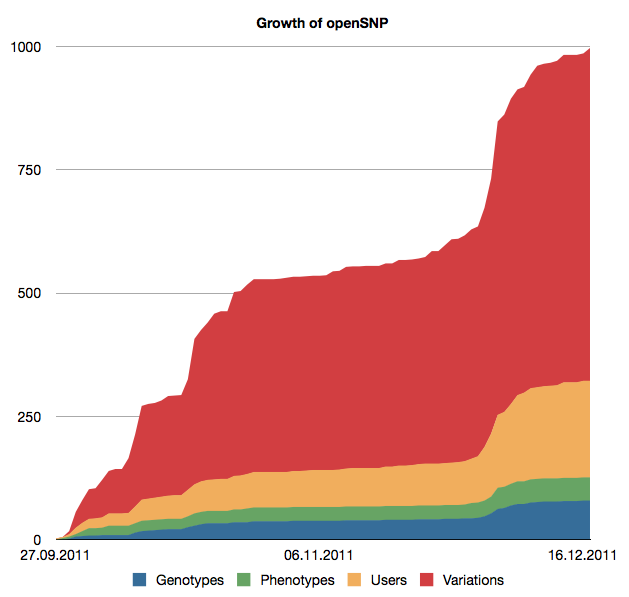
\includegraphics[scale=0.35]{chart_growth.png}
	\end{center}
	\caption{
	{\bf Growth of openSNP.} The increase in numbers for users, genotyping-files, phenotypes and their variation from 27.09.2011 to 16.12.2011 is shown.} 
	\label{Figure1_label}
\end{figure}

\begin{figure}[!ht]
	\begin{center}
		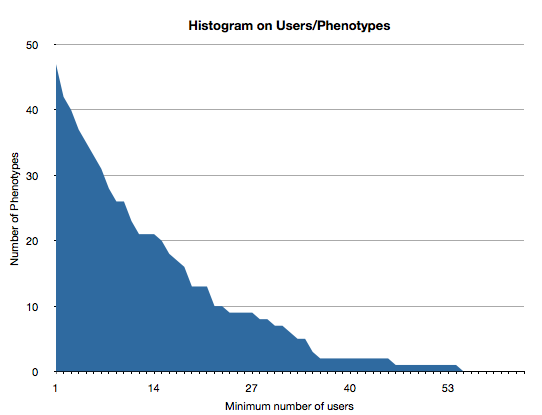
\includegraphics[scale=0.40]{histogram_phenotypes.png}
	\end{center}
	\caption{
	{\bf Histogram of users/phenotype-distribution.} The x-axis shows the minimum number of users who provide information for a phenotype, the y-axis shows how many phenotypes have at least that many users.}
	\label{Figure2_label}
\end{figure}

\begin{figure}[!ht]
	\begin{center}
		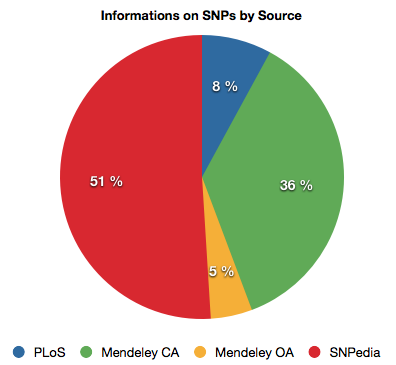
\includegraphics[scale=0.50]{paper_distribution.png}
	\end{center}
	\caption{
	{\bf Distribution of external information gathered for SNPs in the openSNP-database.} Data on PLoS and SNPedia is openly available for every user. Publications on Mendeley are either Open Access (OA) or Closed Access (CA).} 
	\label{Figure3_label}
\end{figure}

\begin{figure}[!ht]
	\begin{center}
		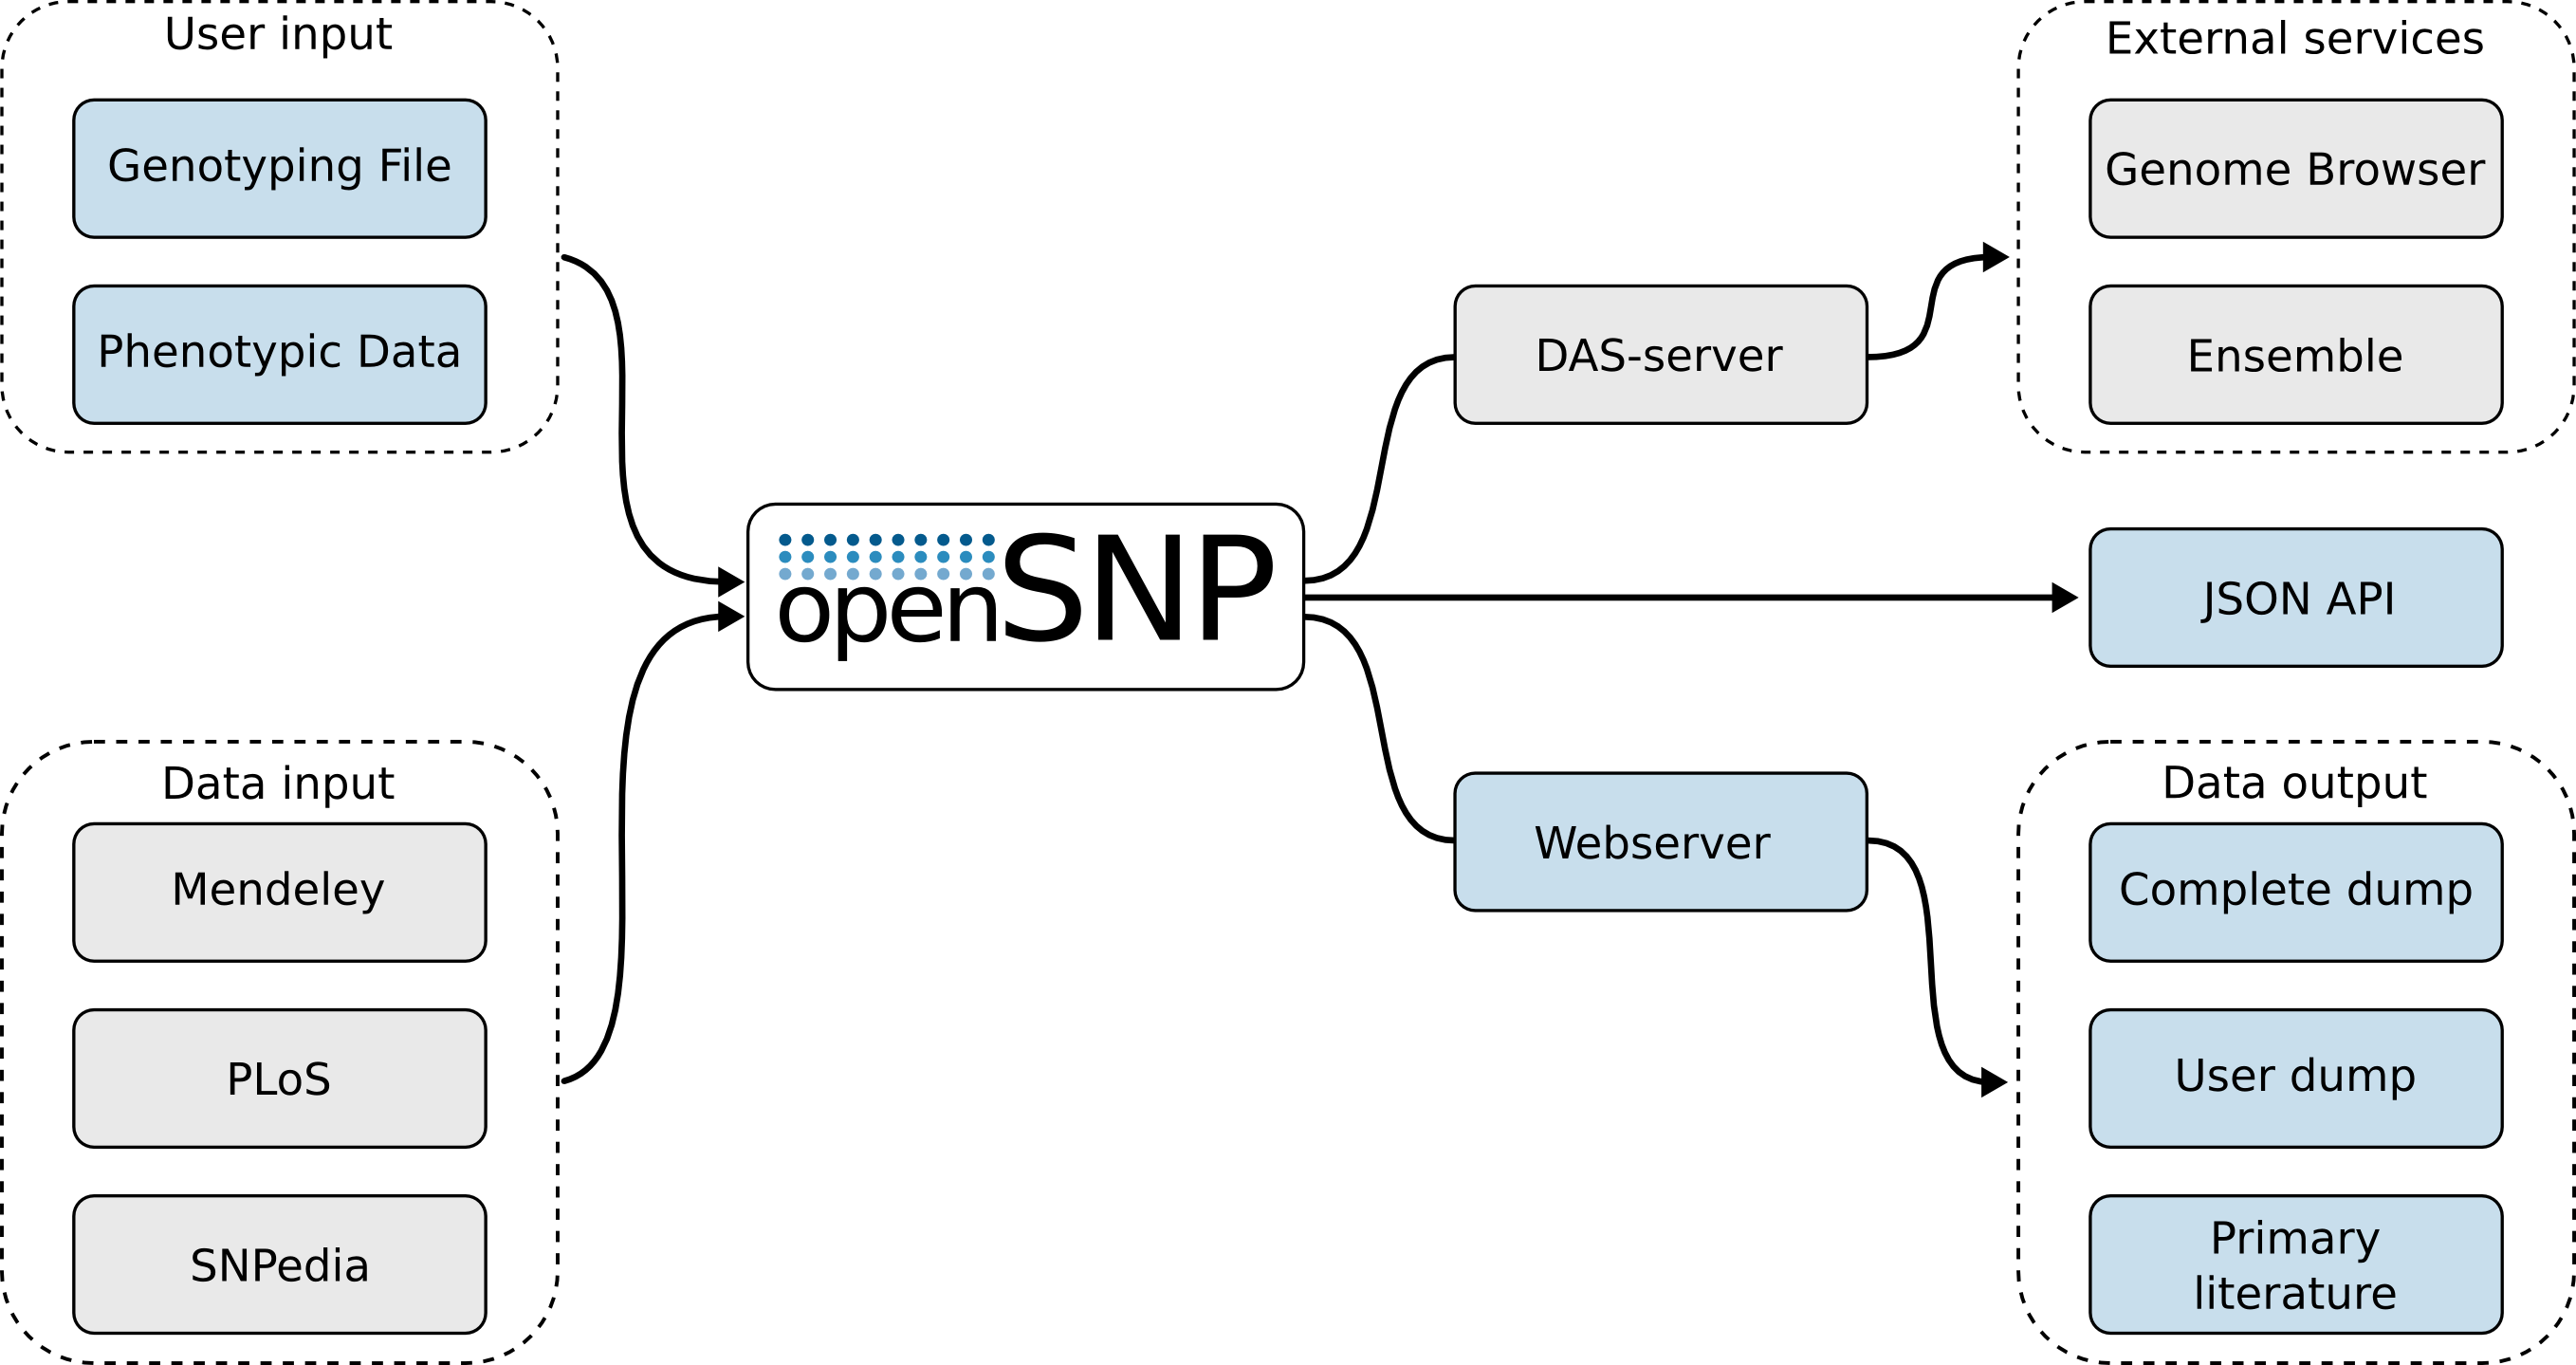
\includegraphics[scale=0.60]{uml_diagram.png}
	\end{center}
	\caption{
	{\bf Flow of data inside openSNP.} External databases and user-provided data are used as input. Output of data is done using the website, the \emph{Distributed Annotation System} and a JSON-API.} 
	\label{Figure4_label}
\end{figure}



%\begin{figure}[!ht]
%\begin{center}
%%\includegraphics[width=4in]{figure_name.2.eps}
%\end{center}
%\caption{
%{\bf Bold the first sentence.}  Rest of figure 2  caption.  Caption 
%should be left justified, as specified by the options to the caption 
%package.
%}
%\label{Figure_label}
%\end{figure}


\section*{Tables}
%\begin{table}[!ht]
%\caption{
%\bf{Table title}}
%\begin{tabular}{|c|c|c|}
%table information
%\end{tabular}
%\begin{flushleft}Table caption
%\end{flushleft}
%\label{tab:label}
% \end{table}

\end{document}
